\chapter{Digital Twin Implementation}\label{ch:implementation}

As introduced in Section~\ref{sec:dt_design}, the \acrshort{dt} developed for this thesis was implemented from scratch, since there is no existing physical twin to model. Therefore, the hypothetical home scenario described in Chapter~\ref{ch:hypothetical_home} served as the basis for the \acrshort{dt} development.

The \acrshort{dt} consists of a \acrfull{rest} \acrfull{api}, which exposes endpoints for accessing and manipulating the data and routines of the home appliances, displaying the energy consumption of the appliances over time, and simulating the effects of adding new routines and resolving potential conflicts with the existing ones. The \acrshort{rest} \acrshort{api} enables the separation of the \acrshort{dt} logic from the user interface, and allows the \acrshort{dt} to be integrated with various clients, such as web applications, mobile applications, and other services. A web application was also developed in this thesis to demonstrate the functionalities of the \acrshort{dt}.

The \acrshort{dt} implementation involved some simplifications and assumptions, which are left for future work to address. First, the \acrshort{dt} operates on a daily basis, from 00:00 to 23:59, and assumes that the routines are repeated every day under the same conditions. This also means that, in circumstances where the \acrshort{dt} uses dates and times in input or output values, the date part is not significant. Second, the \acrshort{dt} only tracks the state of the appliances based on the routines and does not account for the manual activation of the appliances by the users. Third, the \acrshort{dt} relies on static files to provide the information about the routines and appliances in the home and does not update them to reflect the changes in the physical twin. These limitations stem from the fact that there \acrshort{dt} is no physical twin to mirror yet.

The code for the \acrshort{dt} implementation is available with an MIT license on a GitHub repository\footnote{\url{https://github.com/LucaCtt/digital_twin}}.

\newpage

\section{REST API}

An \acrfull{api} is a software interface that defines how different applications or components can communicate and exchange data. It can be seen as a contract that specifies the format and content of the requests and responses between an information provider and an information user~\parencite{redhatinc.WhatRESTAPI2020}.

\acrfull{rest} is an architectural style for designing distributed hypermedia systems that use the HTTP protocol to enable scalable web services. It was first proposed by Roy Fielding in his doctoral dissertation~\parencite{fieldingArchitecturalStylesDesign2000}. The core idea of \acrshort{rest} is to model the system as a collection of resources, which are uniquely identified by URIs and can be accessed and modified using a predefined set of operations~\parencite{framlingProductAgentsHandling2003}.

For an \acrshort{api} to be considered \acrshort{rest}ful, it has to conform to these criteria~\parencite{redhatinc.WhatRESTAPI2020,fieldingArchitecturalStylesDesign2000}:
\begin{itemize}
    \item A client-server architecture that separates the concerns of the clients, servers, and resources, and handles the requests through HTTP.
    \item Stateless communication, meaning that each request is independent and does not rely on any previous or future requests, and no client information is stored on the server side.
    \item Cacheable data that improves the performance and efficiency of the client-server interactions.
    \item A uniform interface that ensures a consistent and standardized way of transferring data between the components, using formats such as XML, JSON, or plain text. This thesis uses JSON, which is a popular and lightweight format that is easy to read and write.
    \item A layered system that abstracts the complexity of the system by hiding the details of each type of server (such as security, load-balancing, etc.) involved in the data retrieval process from the client.
    \item Code-on-demand (optional): the capability of sending executable code from the server to the client upon request, enhancing the functionality of the client.
\end{itemize}

\subsection{Implementation}

The \acrshort{dt} \acrshort{api} is built with Python 3.11, using the FastAPI\footnote{\url{https://fastapi.tiangolo.com/}} library, which is a fast and easy-to-use web framework for creating \acrshort{api}s. The FastAPI library is based on the Starlette\footnote{\url{https://www.starlette.io/}} framework, which is a lightweight \acrfull{asgi} toolkit for developing high-performance services. This enables the \acrshort{dt} \acrshort{api} to handle concurrent requests and to be scalable and maintainable.

FastAPI also supports the automatic generation of OpenAPI documentation, which is a standard for describing \acrshort{rest} \acrshort{api}s. Figure~\ref{fig:backend_swagger} shows an example of such documentation, which is rendered using the Swagger UI\footnote{\url{https://swagger.io/tools/swagger-ui/}}, a tool for exploring and testing the \acrshort{rest} \acrshort{api} resources, based on the OpenAPI specification. The documentation lists all the endpoints, the methods, and the parameters for each endpoint. The UI also shows the possible responses for each endpoint and detailed information about the response format. Moreover, the documentation allows the user to interact with the \acrshort{api} directly from the browser, by sending requests to the endpoints and receiving responses.

\begin{figure}
    \centering
    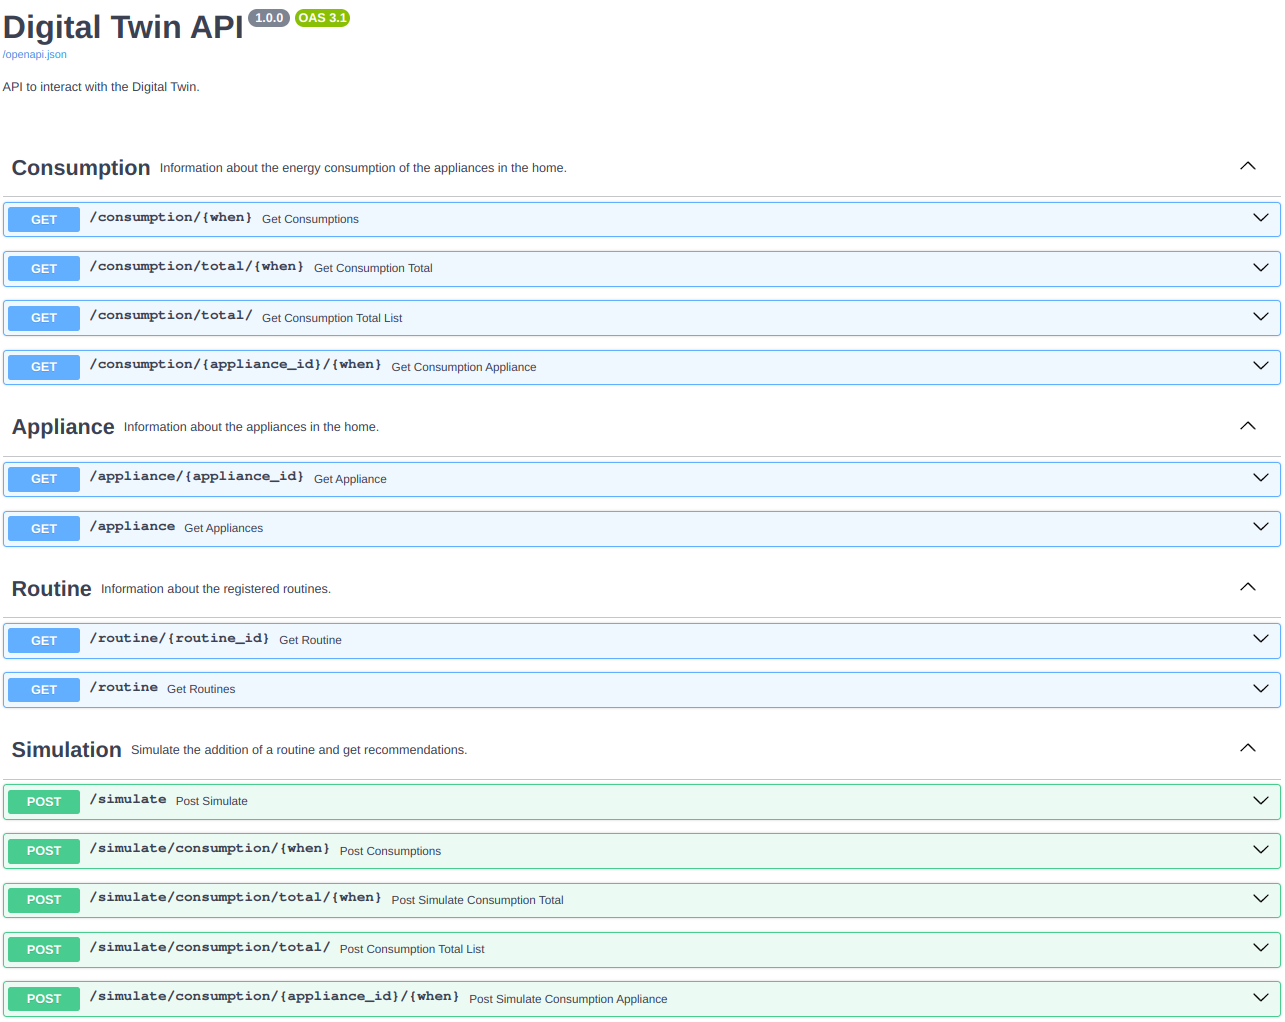
\includegraphics[width=\textwidth]{images/backend_swagger.png}
    \caption{Backend documentation generated by FastAPI}
    \label{fig:backend_swagger}
\end{figure}

Table~\ref{tab:rest_api_endpoints} lists all the endpoints of the \acrshort{dt} \acrshort{api}. The \acrshort{dt} \acrshort{api} offers endpoints to access and modify the data and routines of the home appliances, display the energy consumption of the appliances over time, and simulate the impact of adding new routines and resolving potential conflicts with the existing ones. The \acrshort{dt} \acrshort{api} can simulate the addition of a new routine, evaluate the conflicts with the current routines, and provide suggestions and errors to the user. 

\begin{table}
    \centering
    \resizebox{\textwidth}{!}{%
        \begin{tblr}{ll>{\raggedright}p{.18\textwidth}p{.18\textwidth}lp{.5\textwidth}}
            \hline
            Endpoint                    & Method & Path parameters             & Query Parameters        & Body parameters     & Description                                                                                                                         \\ \hline
            /& GET    & &                         &                     & Displays the \acrshort{api} documentation using Swagger UI.                                           \\ \hline[dashed]
            /consumption                & GET    & Date and time               &                         &                     & Returns a list of energy consumption values of all appliances at the given date and time.                                           \\
            /consumption                & GET    & Appliance id, date and time &                         &                     & Returns the energy consumption value of the given appliance at the given date and time.                                             \\
            /consumption/total          & GET    &                             & List of dates and times &                     & Returns the list of total energy consumption of all appliances at the given dates and times.                                        \\
            /consumption/total          & GET    & Date and time               &                         &                     & Returns the total energy consumption of all appliances at the given date and time.                                                  \\ \hline[dashed]
            /appliance                  & GET    &                             &                         &                     & Returns the list of all appliances                                                                                                  \\
            /appliance                  & GET    & Appliance id                &                         &                     & Returns a specific appliance                                                                                                        \\ \hline[dashed]
            /routine                    & GET    &                             &                         &                     & Returns the list of all routines                                                                                                    \\
            /routine                    & GET    & Routine id                  &                         &                     & Returns a specific routine                                                                                                          \\ \hline[dashed]
            /simulate                   & POST   &                             &                         & Routine to simulate & Simulates the addition of a routine and returns a list of recommendations and errors (if any)                                       \\
            /simulate/consumption       & POST   & Date and time               &                         & Routine to simulate & Simulates the addition of a routine and returns a list of energy consumption values of all appliances at the given date and time    \\
            /simulate/consumption       & POST   & Appliance id, date and time &                         & Routine to simulate & Simulates the addition of a routine and returns the energy consumption value of the given appliance at the given date and time      \\
            /simulate/consumption/total & POST   & Date and time               &                         & Routine to simulate & Simulates the addition of a routine and returns the list of total energy consumption of all appliances at the given dates and times \\
            /simulate/consumption/total & POST   &                             & List of dates and times & Routine to simulate & Simulates the addition of a routine and returns the total energy consumption of all appliances at the given date and time           \\ \hline
        \end{tblr}%
    }
    \caption{Endpoints of the \acrshort{dt}'s REST API}
    \label{tab:rest_api_endpoints}
\end{table}

\subsection{Example of Requests}

\begin{lstlisting}[language=plain,caption={Shape of the \acrshort{api} responses},label=code:api_response_shape,float,floatplacement=H]
{
    value[s]: ...
    error: {
        message: "...",
        context: {
            ...
        }
    }
}
\end{lstlisting}

The \acrshort{api} returns responses in a standardized format, as shown in Code Sample~\ref{code:api_response_shape}. The format includes a \textit{value} field for single-value responses, or a \textit{values} field for multi-value responses. The format may also include an \textit{error} field, which contains a \textit{message} field with an error description, and a \textit{context} field with additional error details.

\begin{lstlisting}[language=numbered,caption={Response to HTTP GET request to the \textit{/consumption/total} endpoint},label=code:api_response_consumption,float,floatplacement=H]
{
  value: 1578,
  error: null,
}
\end{lstlisting}

A \texttt{GET} request to the \texttt{/consumptions/total/2024-02-25T16:00} endpoint returns the total energy consumption of all appliances at 16:00 of the current day (the date part of the string is ignored), as shown in Code Sample~\ref{code:api_response_consumption}. The response has a \texttt{value} field, with the total energy consumption in watts, and a \texttt{null} error field.

\begin{lstlisting}[language=numbered,caption={Response to HTTP POST request to the \texttt{/simulate} endpoint},label=code:api_response_simulate,float,floatplacement=H]
{
  values: [
    {
      "message": "Disable routine \"Wash Everything\"",
      "context": {
        "type": "DISABLE_ROUTINE",
        "routine_id": 3
      }
    },
    {
      "message": "Change start time of routine \"Party Time\"",
      "context": {
        "type": "CHANGE_START_TIME",
          "routine_id": 32,
          "when": "08:00"
      }
    }
  ],
  error: {
    "message": "Power consumption of the house is greater than 3.0kW at 09:59. This can cause a power cut-off.",
    "context": {
      "when": "09:59",
      "max_power": "3000"
    }
  }
}
\end{lstlisting}

A \texttt{POST} request to the \texttt{/simulate} endpoint with a routine in the body simulates the addition of that routine, and returns a list of recommendations and errors. The response to a request with a routine that increases the total consumption of the home above 3kW is shown in Code Sample~\ref{code:api_response_simulate}. The response has a \texttt{values} field, with a list of recommendations, and an \texttt{error} field. In this case, the response recommends changing the start time of the routine or to disable a routine that consumes a lot of energy, and reports an error that the power consumption exceeds the maximum limit. The method for evaluating the conflicts and generating the recommendations and errors is explained in detail in Section~\ref{sec:simulation}.

\section{Configuration}

\begin{lstlisting}[language=json,caption={Example of a configuration file.},label=code:configuration,float,floatplacement=H]
[energy]
max_power = 3
energy_rates_number = 2
energy_rates_prices = [
    0.131870,
    0.111492,
]

[database]
type = "json"
appliances_dir = "json/appliances"
routines_dir = "json/routines"
test_routines_dir = "json/test_routines"
\end{lstlisting}

The \acrshort{dt} supports several configuration parameters, set by a configuration file. The file must be written in TOML, and its location is specified by the \texttt{CONFIG\_PATH} environment variable. The configuration file contains the following information:
\begin{itemize}
    \item \texttt{energy}: energy-related parameters.
          \begin{itemize}
              \item \texttt{max\_power}: the maximum power consumption, in kW;
              \item \texttt{energy\_rates\_number}: the number of energy tariffs, e.g. 2 for dual-rate;
              \item \texttt{energy\_rates\_prices}: the cost of each energy tariff, in \texteuro/kWh.
          \end{itemize}
    \item \texttt{database}: database-related parameters.
          \begin{itemize}
              \item \texttt{type}: the type of database, only JSON is supported at the moment;
              \item \texttt{appliances\_dir}: the directory where the appliances JSON files are stored;
              \item \texttt{routines\_dir}: the directory where the routine JSON files are stored;
              \item \texttt{test\_routines\_dir}: the directory where the JSON files for the test routines are stored;
          \end{itemize}
\end{itemize}

The \acrshort{dt} supports up to three energy tariffs (F1, F2, F3), as defined by the \acrfull{arera} in the Delibera n.181/06\footnote{\url{https://www.arera.it/atti-e-provvedimenti/dettaglio/06/181-06} (visited on 2024, February 22)}. The tariffs vary according to the time and the day of the week, as shown in Figure~\ref{fig:costs_matrix}. The peak F1 goes from 8:00 to 19:00, Monday to Friday. The intermediate tariff F2 goes from 7:00 to 8:00 and from 19:00 to 23:00, Monday to Friday, and from 7:00 to 23:00 on Saturday. The off-peak tariff F3 goes from 23:00 to 7:00, Monday to Saturday, and from 23:00 to 24:00 on Sunday. The number of tariffs can be lower than three, depending on the contract with the energy provider. If only two tariffs are available, F2 and F3 are merged into a single tariff F23.

\begin{figure}
    \centering
    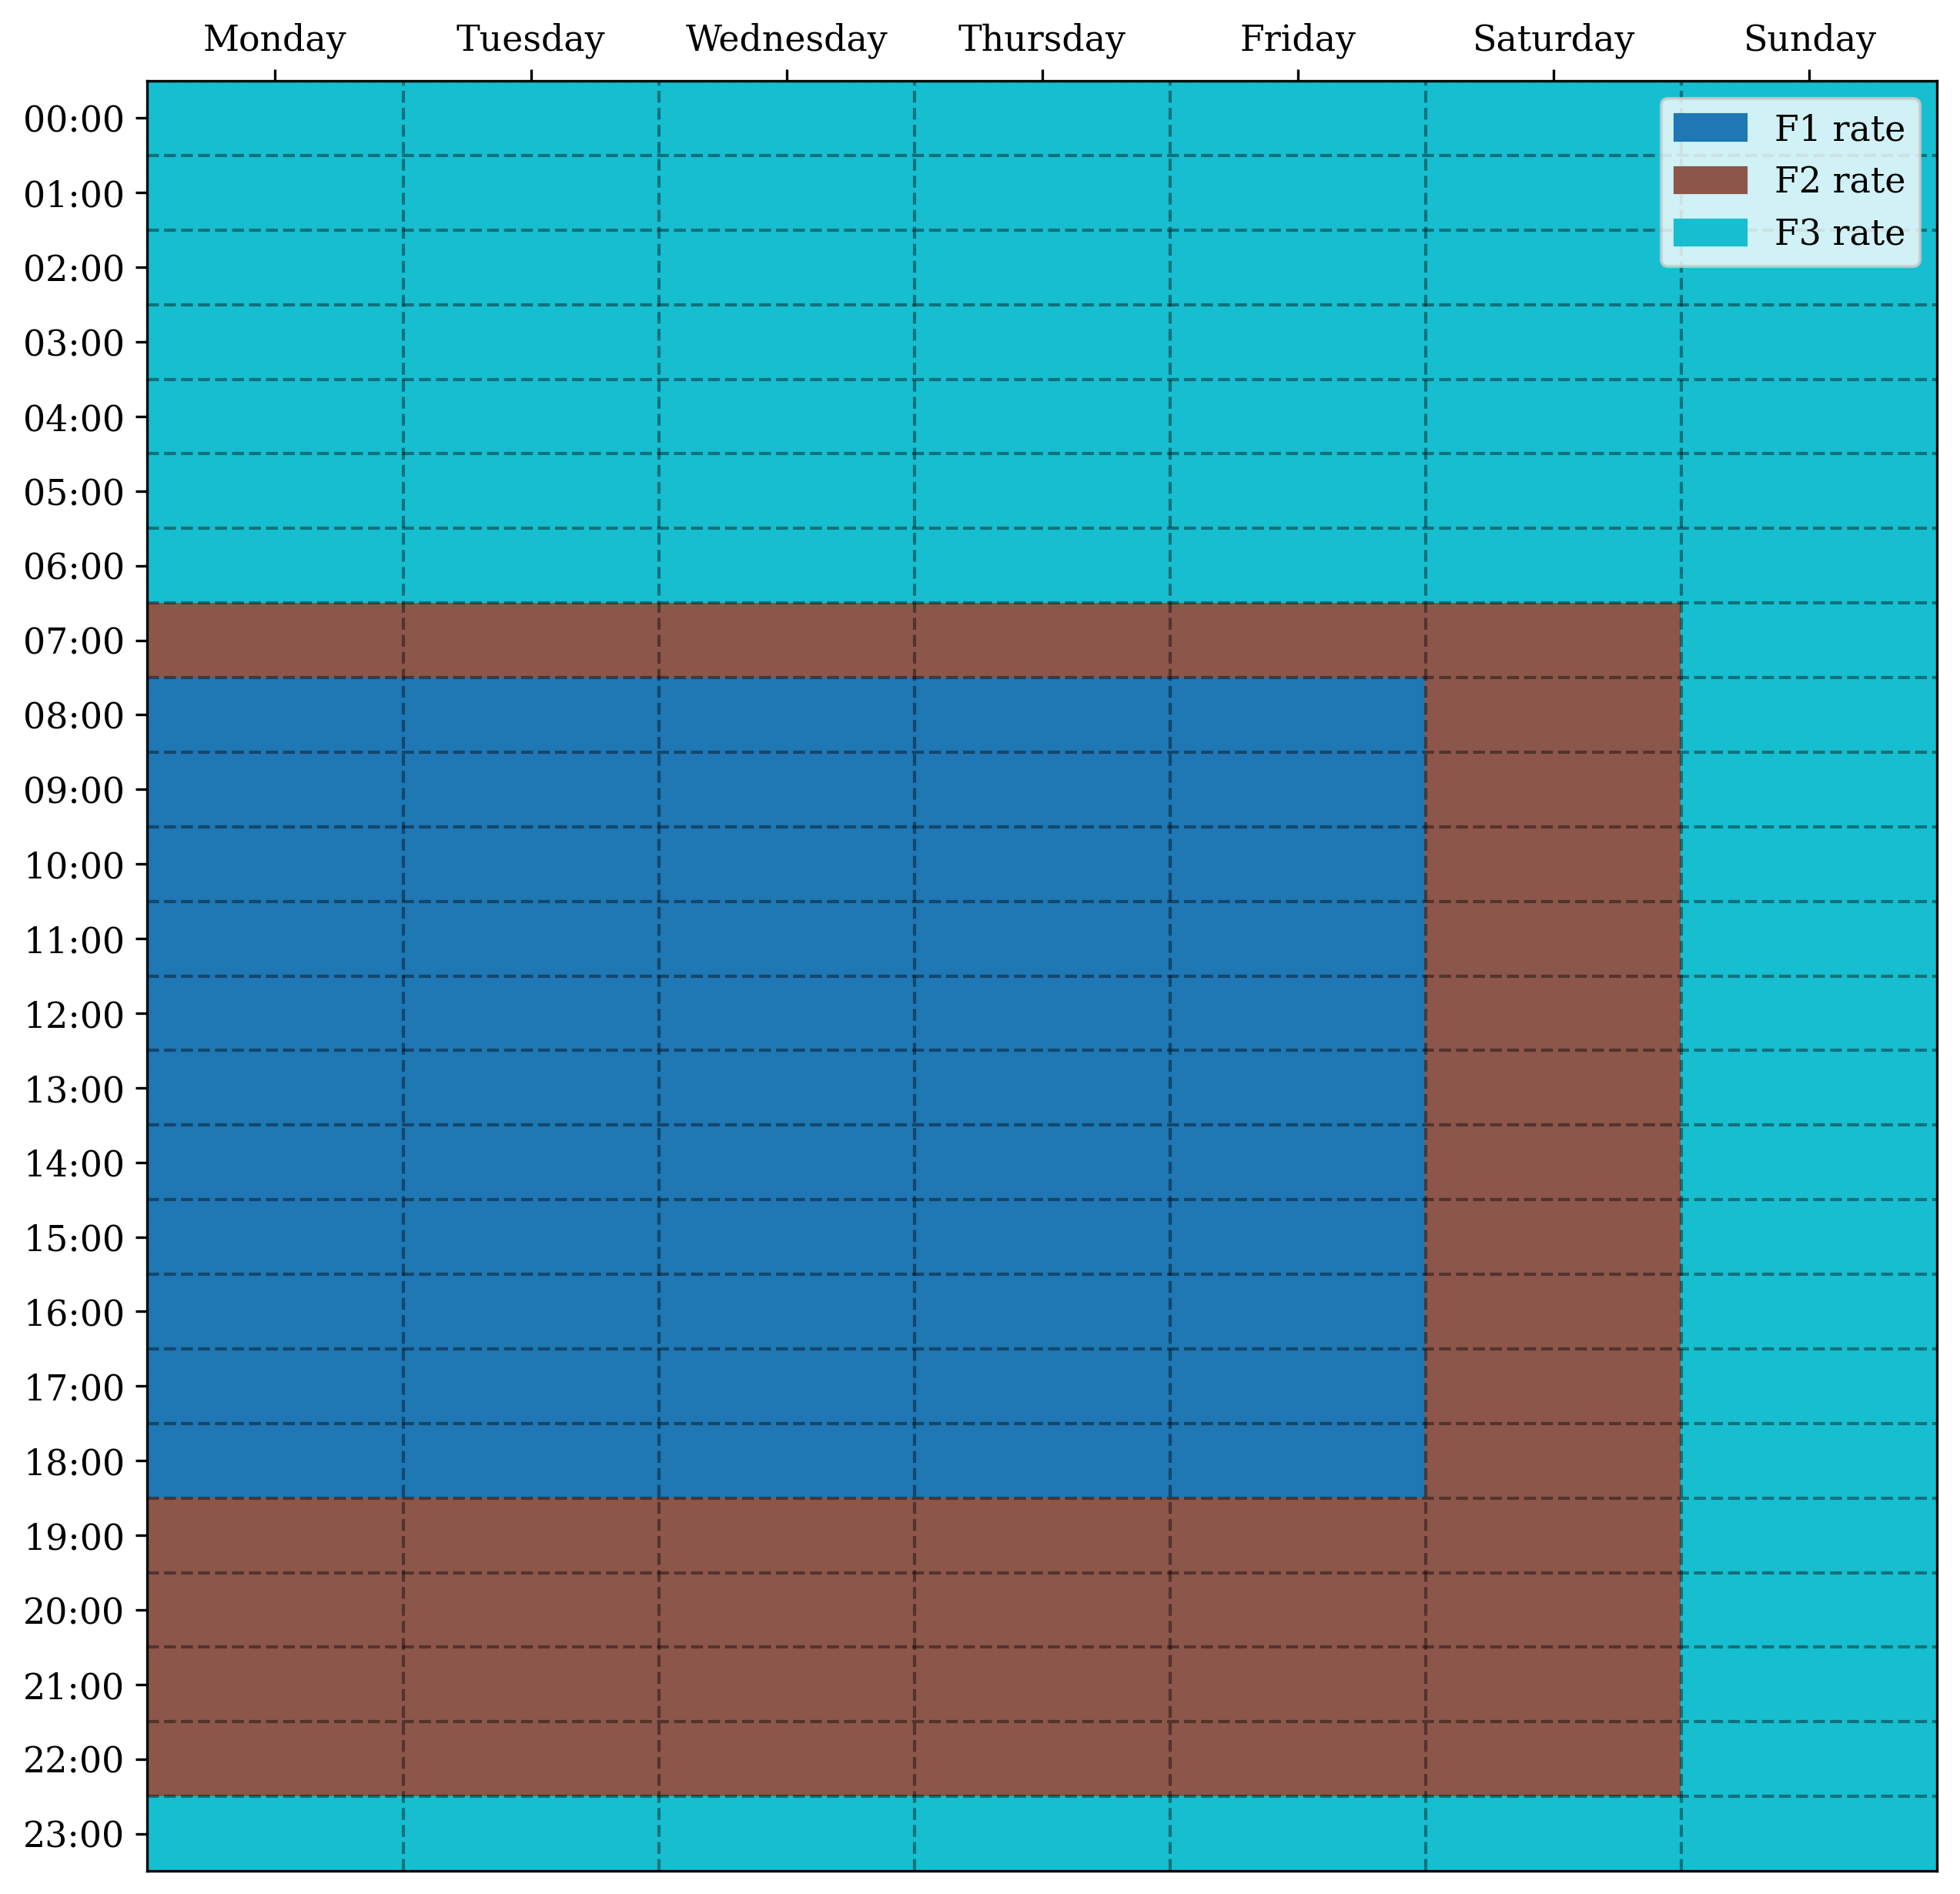
\includegraphics[width=0.9\textwidth]{images/costs.png}
    \caption[Electricity tariffs applied in italy for every day of the week]{Electricity tariffs applied in italy for every day of the week. F1 is the peak rate, F2 is the mid-level, and F3 is off-peak}
    \label{fig:costs_matrix}
\end{figure}

The configuration used for the development of the \acrshort{dt} is shown in Code Sample~\ref{code:config}. Two energy tariffs are used with prices based on the \acrfull{pun} values for December 2023, which are the Single National Price. The \acrshort{pun} is calculated by the \acrfull{gme}\footnote{\url{https://www.mercatoelettrico.org/En/default.aspx} (visited on 2024, February 22)}, as the weighted average of the prices of the energy markets, and is used as a reference for the energy costs in Italy. The maximum power consumption is set to 3kW, which is the standard limit for the power supply in Italy.

\section{Appliance and Routine Data}

The appliances in the hypothetical home and the routines defined by the end users are represented by JSON files. Code Samples~\ref{code:appliance_dish_washer} and~\ref{code:appliance_washing_machine} show the JSON files for the dishwasher and the washing machine, respectively. Each JSON file includes the following information:
\begin{itemize}
    \item \texttt{id}: a unique integer identifier for the appliance;
    \item \texttt{device}: the appliance type, such as \textit{dishwasher};
    \item \texttt{manufacturer} (optional): the appliance manufacturer, such as \textit{Whirlpool};
    \item \texttt{model} (optional): the appliance model, such as \textit{ADF 555 IX};
    \item \texttt{location}: the room where the appliance is located, such as the \textit{kitchen};
    \item \texttt{modes}: the list of operation modes available for the appliance. Each appliance has at least an \textit{off} mode, which consumes no power. Each mode has the following information:
    \begin{itemize}
        \item \texttt{id}: a unique integer identifier for the mode;
        \item \texttt{name}: the mode name, such as \textit{intensive};
        \item \texttt{power\_consumption}: the average power consumption of the appliance in the mode, in Watts; 
        \item \texttt{default\_duration} (optional): the default duration of the mode, which is used if the user does not specify a duration in the routine. If no default duration is specified, the mode is assumed to be running until the end of the day.
    \end{itemize}
\end{itemize}

\begin{lstlisting}[language=numbered,caption={JSON file describing the dish washer},label=code:appliance_dish_washer,float,floatplacement=H]
{
  "id": 3,
  "device": "dish washer",
  "manufacturer": "Whirlpool",
  "model": "ADG 555 IX",
  "location": "kitchen",
  "modes": [
    {
      "id": 0,
      "name": "off",
      "power_consumption": 0
    },
    {
      "id": 1,
      "name": "daily",
      "power_consumption": 810,
      "default_duration": 10260
    },
    ...	
    {
      "id": 6,
      "name": "pre-wash",
      "power_consumption": 10,
      "default_duration": 660
    }
  ]
}
\end{lstlisting}

\begin{lstlisting}[language=numbered,caption={[JSON file describing the washing machine]JSON file describing the washing machine.},label=code:appliance_washing_machine,float,floatplacement=H]
{
	"id": 15,
	"device": "washing machine",
	"manufacturer": "Zanussi",
	"model": "F1215",
	"location": "bathroom",
	"modes": [
		{
			"id": 0,
			"name": "off",
			"power_consumption": 0
		},
		{
			"id": 1,
			"name": "cotton 90",
			"power_consumption": 2000,
			"default_duration": 8700
		},
		...	
		{
			"id": 7,
			"name": "wool",
			"power_consumption": 450,
			"default_duration": 3300
		}
	]
}
\end{lstlisting}

Code Sample~\ref{code:routine_wash_everything} shows an example of a routine that starts the dishwasher in \textit{intensive} mode and the washing machine in \textit{cotton 90} mode at 14:00. The routine file has the following information:
\begin{itemize}
    \item \texttt{id}: a unique integer identifier for the routine;
    \item \texttt{name}: a name for the routine, such as \textit{wash everything};
    \item \texttt{when}: the time when the routine is executed, in the format \textit{HH:MM};
    \item \texttt{actions}: the list of actions that the routine performs. Each action has the following information:
    \begin{itemize}
        \item \texttt{id}: a unique integer identifier for the action;
        \item \texttt{appliance\_id}: the ID of the appliance that the action affects;
        \item \texttt{duration} (optional): the duration of the mode, in minutes. If not specified, the default duration of the mode is used.
    \end{itemize}
\end{itemize}

\begin{lstlisting}[language=numbered,caption={[Example of a routine with two actions]Example of a routine with two actions.},label=code:routine_wash_everything,float,floatplacement=H]
{
    "id": 5,
    "name": "Wash everything",
    "when": "14:00",
    "enabled": true,
    "actions": [
        {
            "id": 0,
            "appliance_id": 15,
            "mode_id": 1
        },
        {
            "id": 1,
            "appliance_id": 3,
            "mode_id": 1
        }
    ]
}
\end{lstlisting}

\section{Appliance State Modeling}

The \acrshort{dt} can create a \textit{state matrix} of the appliances throughout the day, based on the defined routines. The state matrix tracks the operation mode of each appliance for every minute of the day. It is used to evaluate the conflict scenarios and to simulate the addition of a new routine. Figure~\ref{fig:state_matrix} shows an example of a state matrix, which displays the operation modes of the appliances in the hypothetical home throughout the day, using a predefined set of routines.

\begin{figure}
    \centering
    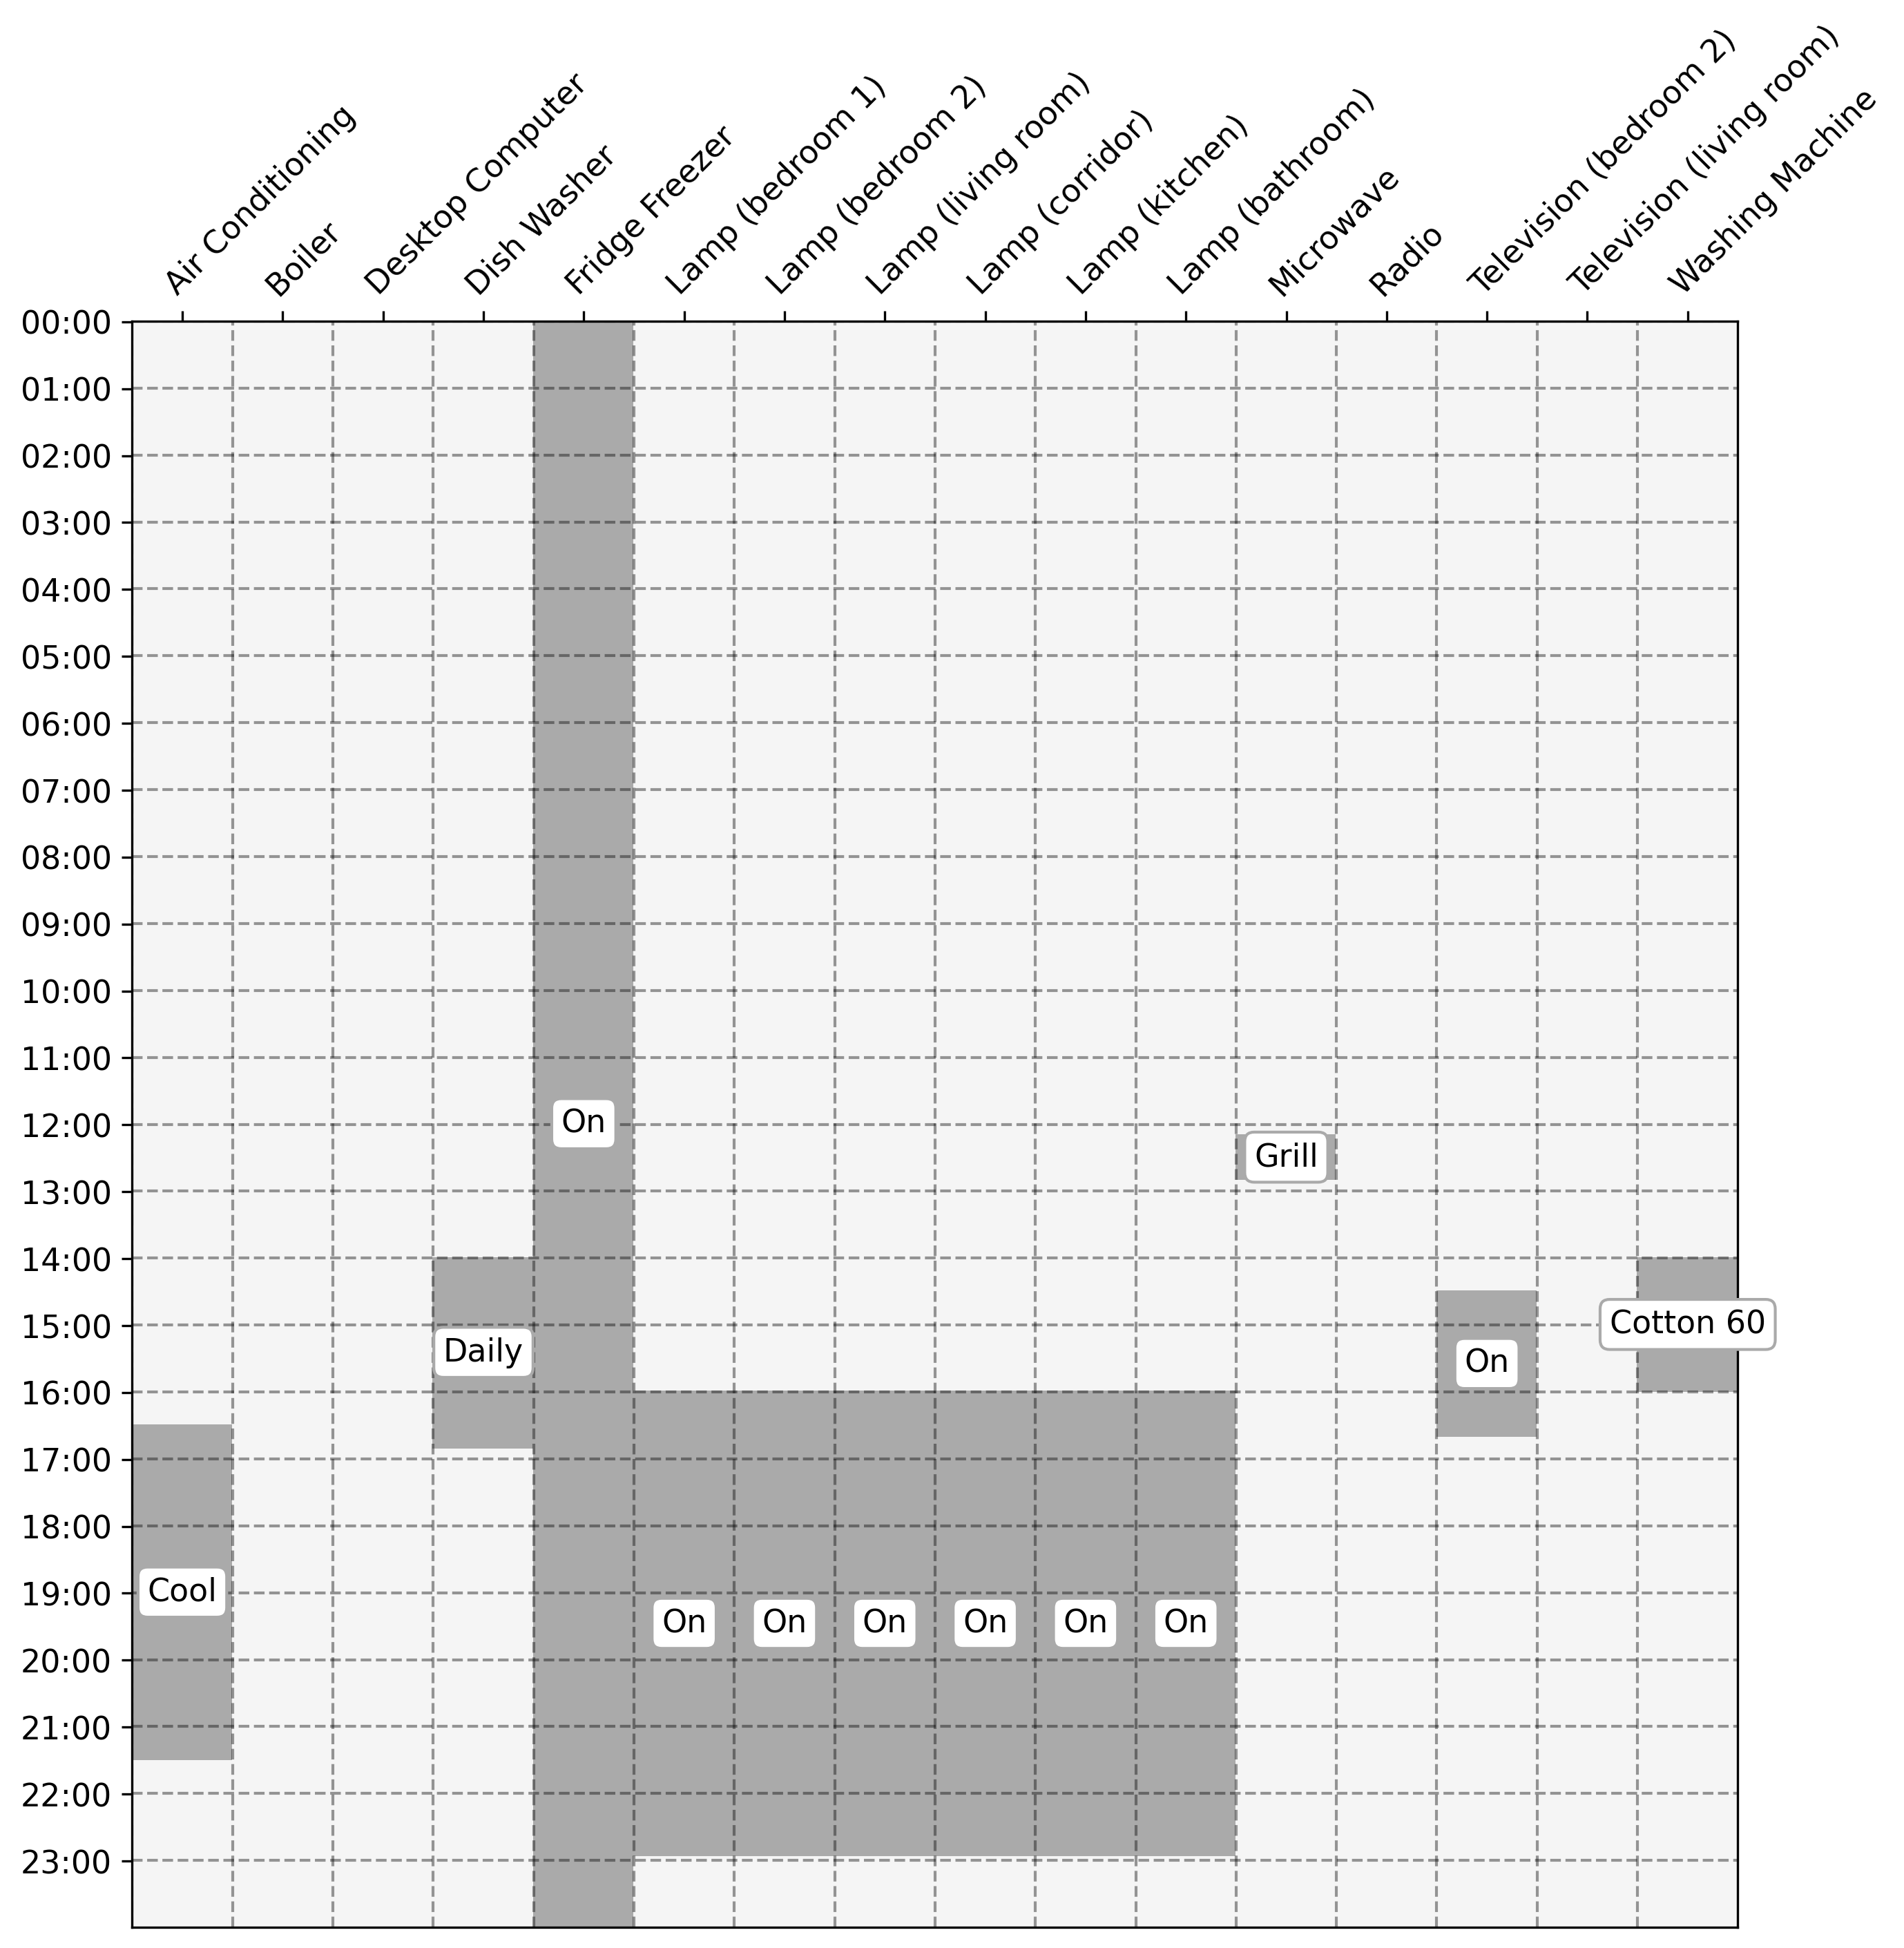
\includegraphics[width=0.9\textwidth]{images/real_matrix.png}
    \caption[Example of a state matrix]{Example of a state matrix. The matrix shows the operation modes of the appliances in the hypothetical home throughout the day, using a predefined set of routines}
    \label{fig:state_matrix}
\end{figure}

The state matrix is implemented using the \texttt{ndarray} class from the NumPy library~\parencite{harrisArrayProgrammingNumPy2020}, which is a n-dimensional array of integers. According to the Numpy N-Dimensional Array Reference\footnote{\url{https://numpy.org/doc/1.26/reference/arrays.ndarray.html}}, an instance of the \texttt{ndarray} class consists of a contiguous one-dimensional memory segment, which is combined with an indexing scheme to represent multidimensional arrays, mapping integers to the various elements that compose the memory block.

Each row of the matrix corresponds to a minute of the day, and each column corresponds to an appliance, by using the appliance ID as the column index. For instance, the first column of the matrix (index $0$) corresponds to the appliance with index 0. The value of each cell is the ID of the operation mode in which the appliance is set at that minute. Given that in a day there are $24 \times 60 = 1440$ minutes, and the hypothetical home has 15 appliances, the state map is a $1440 \times 15$ matrix. The matrix type is \textit{uint8}, which can store integers from $0$ to $255$, which is sufficient to store the IDs of the operation modes of the appliances. The state matrix uses $1440 \times 15 \times 8 = 172800$ bits of memory, which corresponds to about $21$ kilobytes.

The state matrix makes it straightforward to calculate the consumption of an appliance at any time of the day. It is enough to index the matrix with the minute of the day and the appliance ID. The resulting value is the ID of the operation mode of the appliance at that time, and it can be used to get the energy consumption of the mode from the appliance's JSON file. To get the total energy consumption at any time of the day, it is enough to add the energy consumption of the individual appliances at that time.

\section{Simulation of New Routines}\label{sec:simulation}

When simulating the addition of a new routine, it may cause a conflict with the existing routines. It is assumed that the existing routines are already consistent and conflict-free. The \acrshort{dt} is capable of evaluating such conflicts and producing \textit{errors} or \textit{recommendations}, or both. An error occurs when a conflict creates an inconsistency among the routines, e.g. when two routines include actions that contradict each other, or that put the power draw over a maximum limit. Errors halt the simulation and prevent further evaluation. Recommendations are either warnings about minor conflicts that do not affect the consistency, or suggestions to improve the user experience or save energy. A recommendation does not interrupt the simulation and allows for further evaluation. This means that the digital twin can provide multiple recommendations for different conflicts, but at most one error is returned at a time.

The expected conflict scenarios are the following:
\begin{enumerate}[label={\textit{S\arabic*.}}, leftmargin=3.5em]
    \item \textit{An appliance has conflicting operation modes in the same time interval}. This occurs when a simulated routine assigns an appliance a different operation mode than the one assigned by the existing routines in the same time interval. If the simulated routine assigns the same operation mode as the existing routines, there is no conflict. For instance, the AC is set to \textit{heat} from 8:00 to 12:00. A simulated routine that sets the AC to \textit{cold} from 10:00 to 11:00 causes a conflict. The digital twin rejects the simulated routine with an error that specifies the conflicting action and the existing routine and action. It also suggests deactivating the existing routine instead. This may be useful, for example, in weather conditions with sudden temperature changes, where the user may want to adjust the AC temporarily. If the simulated routine does not cause an inconsistency, e.g. it sets the AC to \textit{heat} from 11:00 to 13:00, then the digital twin accepts the simulated routine with a recommendation to modify the existing routine action to set \textit{heat} from 8:00 to 13:00.

    \item \textit{The power consumption exceeds a maximum limit at any time}. The digital twin rejects any routine that causes the power consumption to go beyond the maximum limit at any point. This limit could be the maximum power supply before cut-off, e.g. $3kW$ in Italy. For example, if the microwave is in \textit{microwave mode}, the dishwasher is in \textit{intensive} mode, and the simulated routine sets the washing machine to \textit{cotton 60} mode at 14:00, the digital twin produces an error and advises a better start time for the washing machine.

    \item \textit{A better start time can be determined}. The digital twin tries to find a more economical start time for each action of the simulated routine, using pre-set electricity costs. This is important, for example, if the user has a variable electricity tariff, where it is less expensive to run appliances at night. If the electricity cost is constant throughout the day, this step can be ignored. The digital twin evaluates each action of the simulated routing sequentially, taking into account the best start time of the previous actions. For instance, if the best start time of action 1 of the simulated routine is 15:30, the digital twin should use that as a reference when evaluating action 2.

    \item \textit{An appliance is activated manually by the end user}. This scenario requires the digital twin to monitor the running state of appliances, in addition to the routines. Before executing any routine actions, the digital twin should check for conflicts with scenarios S1 and S2, using the current state of the appliances as well. If the scenarios produce an error, the conflicting actions should be prevented from running. Actions that are conflict-free can still be executed. Any recommendation produced can be displayed to the user to alert them and offer alternatives on what to do.
\end{enumerate}

The implementation of the digital twin developed for this thesis only covers conflicts S1-S4, while conflict S5 is left as a future development.

\begin{figure}
    \centering
    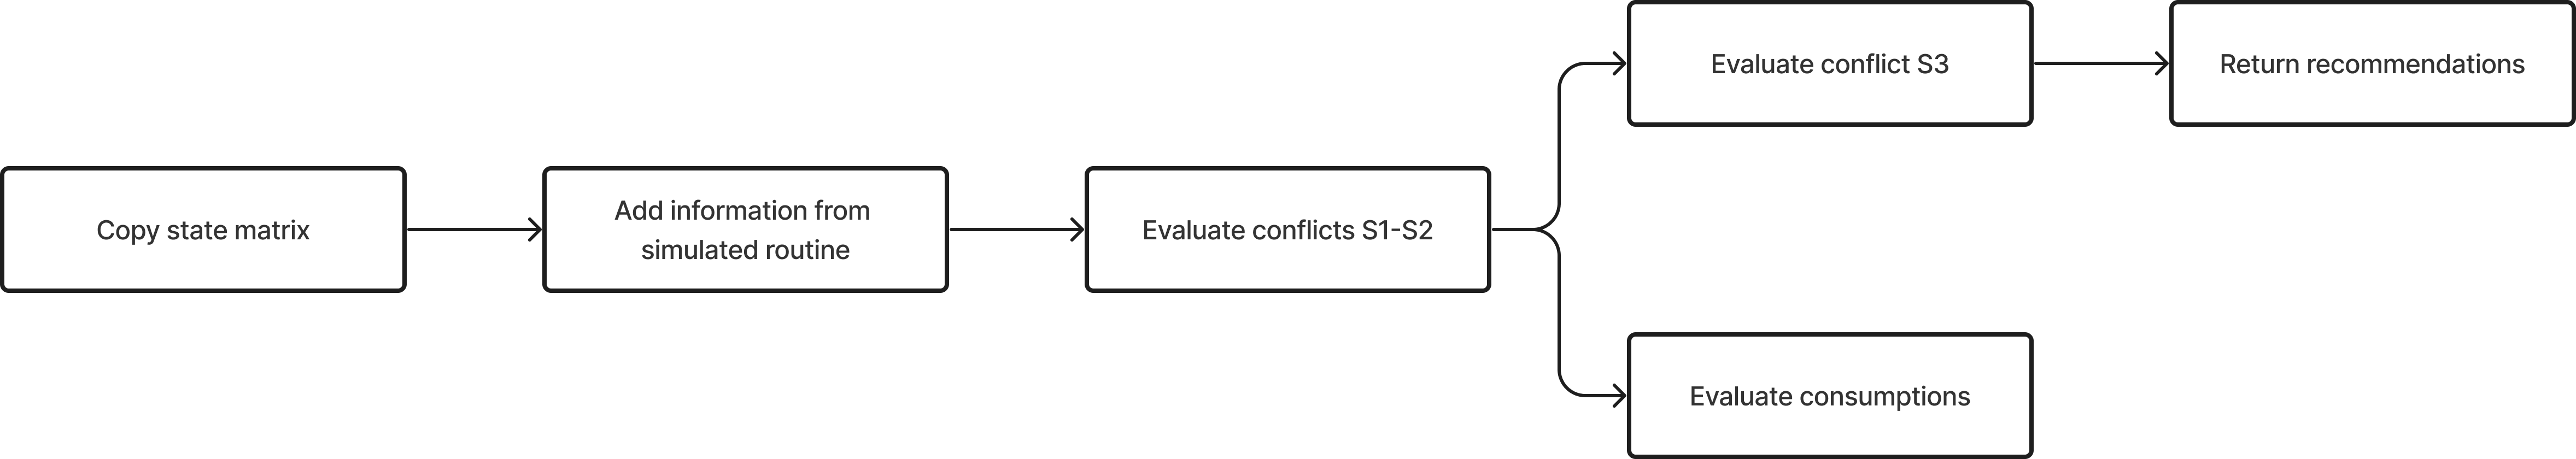
\includegraphics[width=\textwidth]{images/simulation_procedure.png}
    \caption{Simulation procedure}
    \label{fig:simulation_procedure}
\end{figure}

Figure~\ref{fig:simulation_procedure} shows the complete procedure for simulating the addition of a new routine. The procedure starts by creating a copy of the state matrix, using the \texttt{copy} method from NumPy. The new matrix is then updated with the new appliance states from the simulated routine. The procedure then checks for the conflicts described above, and stops if there is an error. Figure~\ref{fig:simulated_consumption_matrix} shows an example of a simulated matrix, which is obtained by adding a new routine to the matrix in Figure~\ref{fig:state_matrix}. The \texttt{/simulate} endpoint of the \acrshort{api} returns the list of recommendations and errors, if any. The other simulation endpoints of the \acrshort{api} do not return any recommendation, but only compute consumption values on the new state matrix. Any error is returned as well.

\begin{figure}
    \centering
    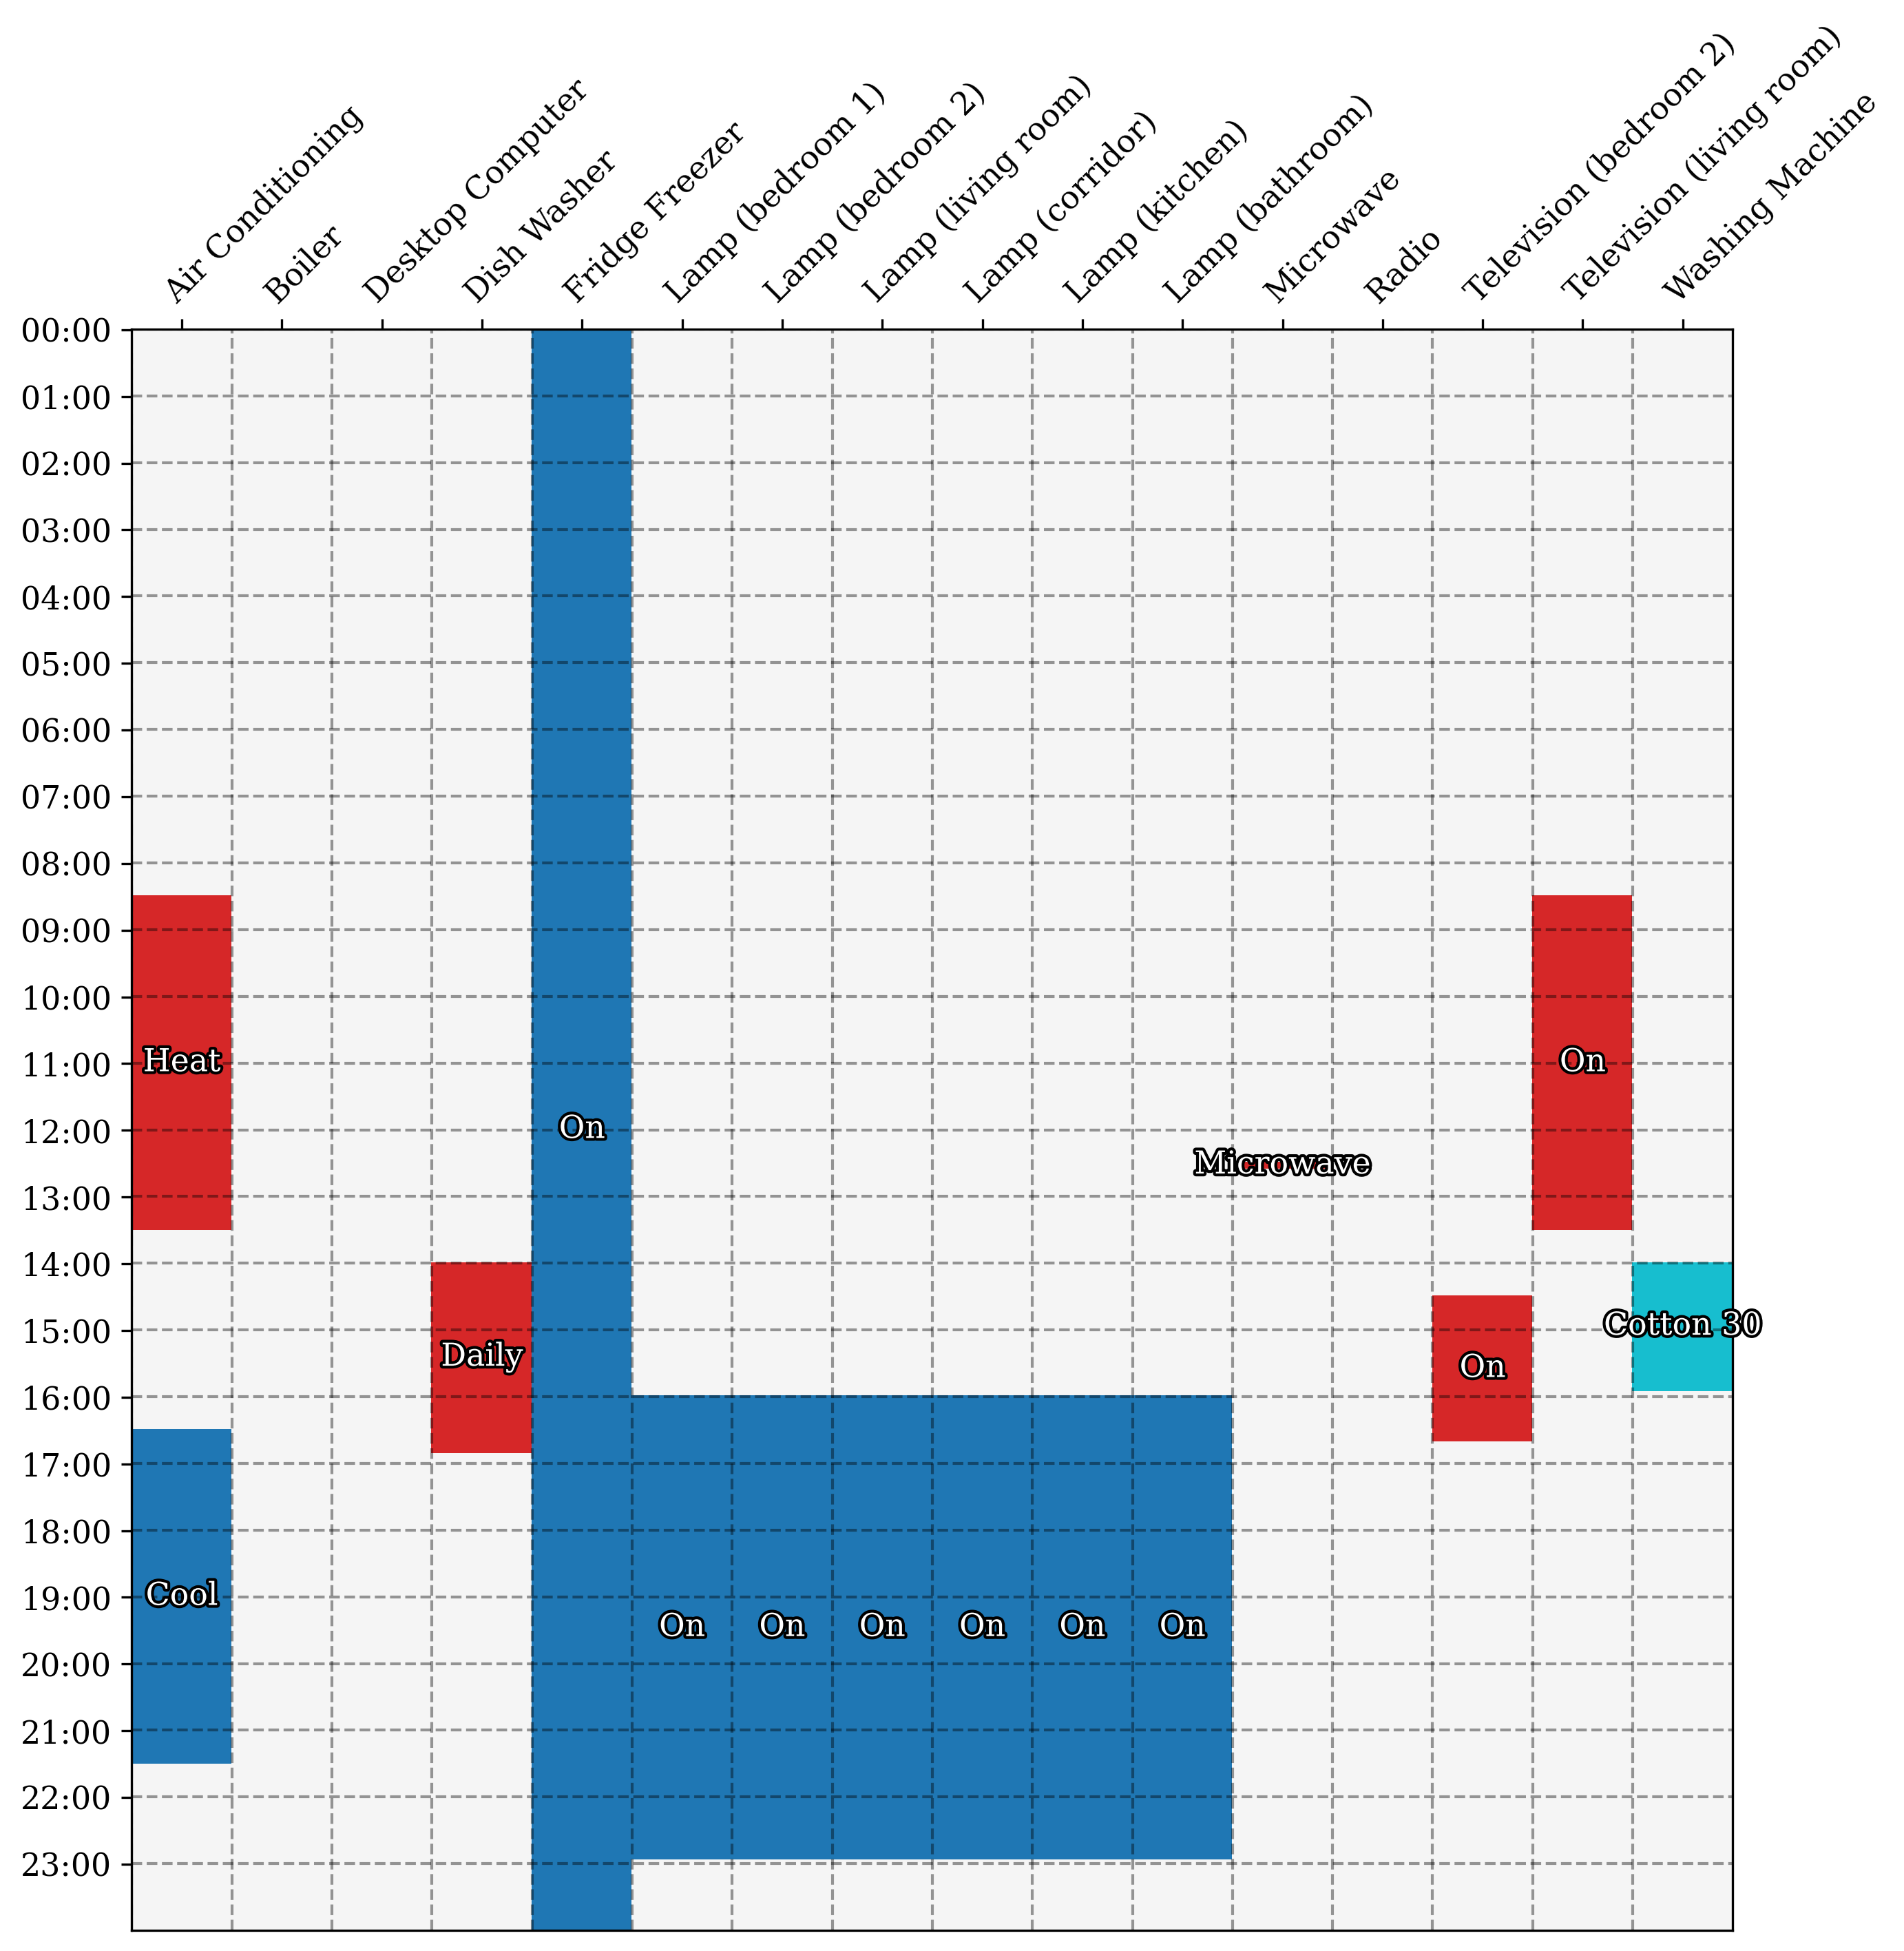
\includegraphics[width=0.9\textwidth]{images/simulated_matrix.png}
    \caption{Simulated matrix}
    \label{fig:simulated_consumption_matrix}
\end{figure}

To find the best start time according to S3, the \acrshort{dt} uses a brute force approach, by evaluating the energy cost of starting the simulated routine at every minute of the day, and choosing the one with the lowest cost. The energy cost of a routine is calculated by adding the cost of starting each action at the chosen time, using the energy rates from the configuration file. This operation is repeated $1440$ times, once for every minute of the day. The \acrshort{dt} then returns the best start time, and the monetary savings of starting the routine at that time. The monetary savings are calculated by comparing the cost of starting the routine at the best start time with the cost of starting the routine at the time given in the routine.

\section{Frontend}

The frontend application demonstrates the functionalities of the \acrshort{dt}, but it is not a fully functional interface for end users. The application displays the energy consumption of appliances during the day, simulates the addition of new routines and checks for possible conflicts with the existing routines. The application also shows the list of appliances and routines in the home.

The application is built using the React\footnote{\url{https://react.dev/}} framework, which is a JavaScript library for creating user interfaces. React is simple and fast, as it uses a component-based architecture, which allows to create complex user interfaces by combining small and isolated pieces of code. The frontend is styled using the Tailwind CSS \footnote{\url{https://tailwindcss.com/}} library, which is a utility-first CSS framework that enables the creation of custom designs without writing custom CSS. The FlowBite\footnote{\url{https://flowbite.com/}} library provides a set of ready-made TailwindCSS components, which also support dark mode.

\begin{figure}
    \centering
    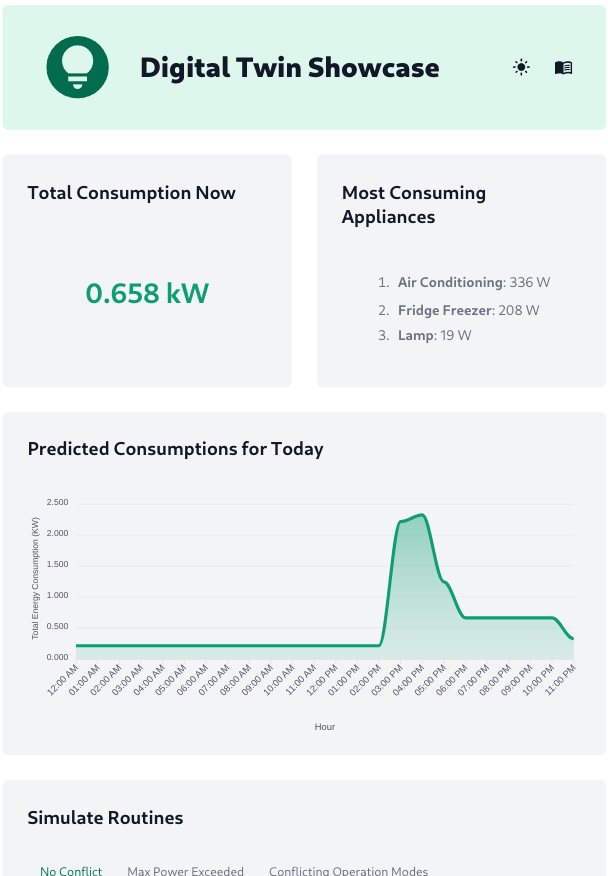
\includegraphics[width=0.8\textwidth]{images/frontend/responsive.png}
    \caption{Display of the website on an iPad Air device}
    \label{fig:frontend_responsive}
\end{figure}

The application is also \textit{responsive}, meaning that it adjusts to different screen sizes, and works on both desktop and mobile devices~\parencite{marcotteResponsiveWebDesign2010}. However, some elements of the page, such as tables, are not very readable on mobile devices. An example of how the website is displayed on a tablet is provided in Figure~\ref{fig:frontend_responsive}. 

\subsection{Header Section}

The header of the frontend application, displayed in Figure~\ref{fig:frontend_header}, contains the the title and logo of the application, which is derived from Material Icons\footnote{\url{https://fonts.google.com/icons}}. There are two buttons on the right side of the header, which enable the user to switch between light and dark modes, and to access the \acrshort{api} documentation.

\begin{figure}
    \centering
    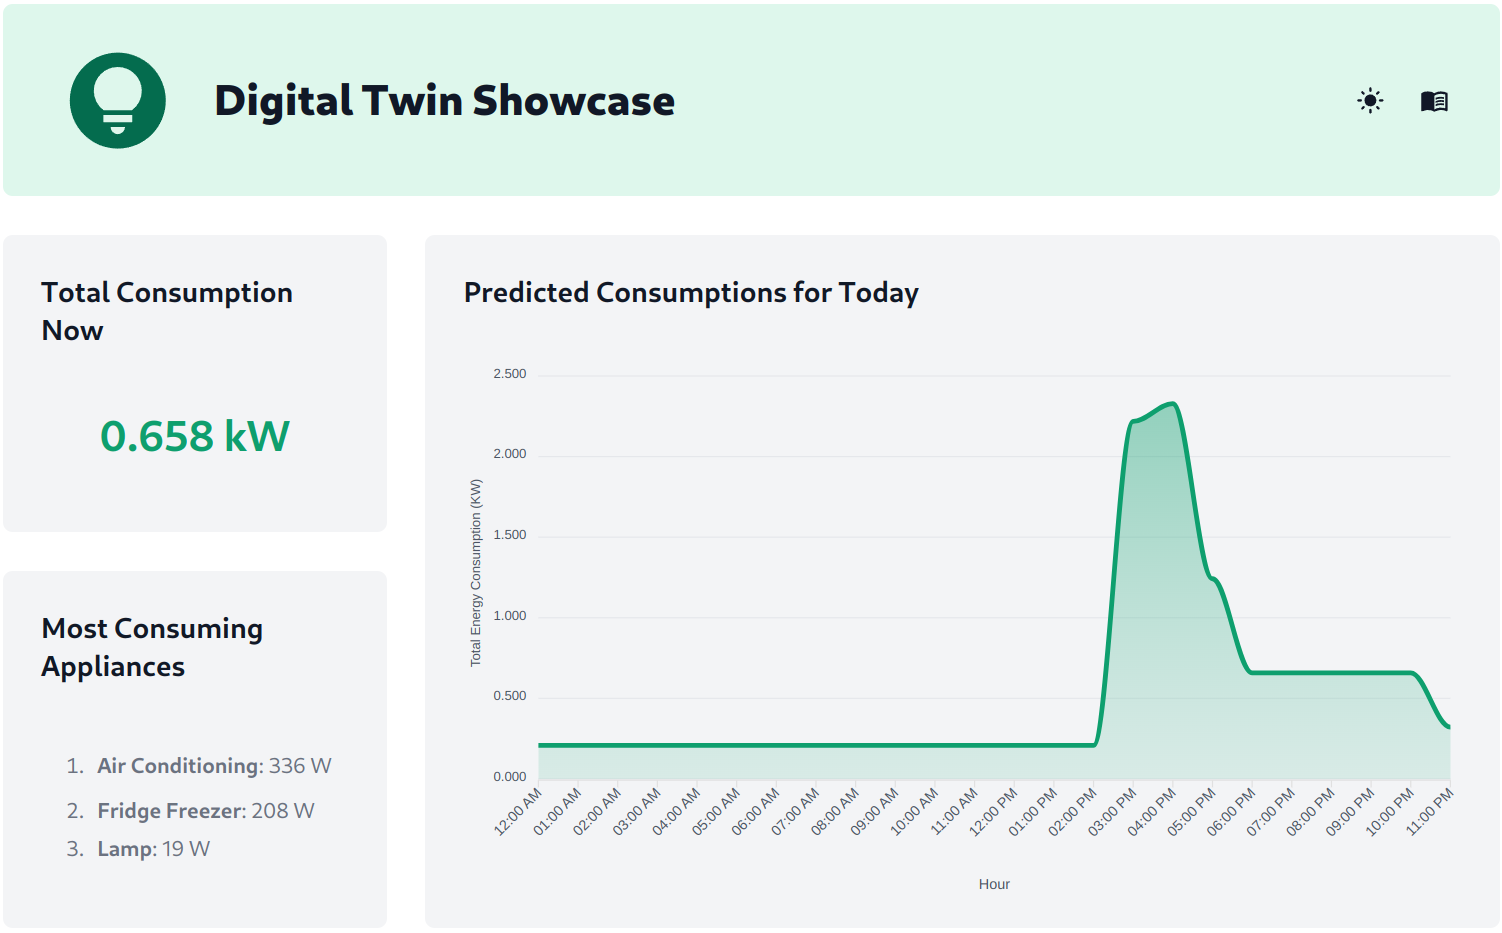
\includegraphics[width=0.9\textwidth]{images/frontend/header.png}
    \caption{Header of the frontend application}
    \label{fig:frontend_header}
\end{figure}

\subsection{Statistics Section}

The statistics section, shown in Figure~\ref{fig:frontend_statistics}, provides various information about the home's energy consumption:
\begin{itemize}
    \item The total power consumption of all appliances at the current time.
    \item The three appliances that consume the most power at the current time, and their respective power consumption values.
    \item A chart that predicts the total power consumption of all appliances throughout the day, based on historical data and machine learning models. The chart is implemented using the ApexCharts\footnote{\url{https://apexcharts.com/}} library, and offers features such as zooming, panning, and tooltips.
\end{itemize}

\begin{figure}
    \centering
    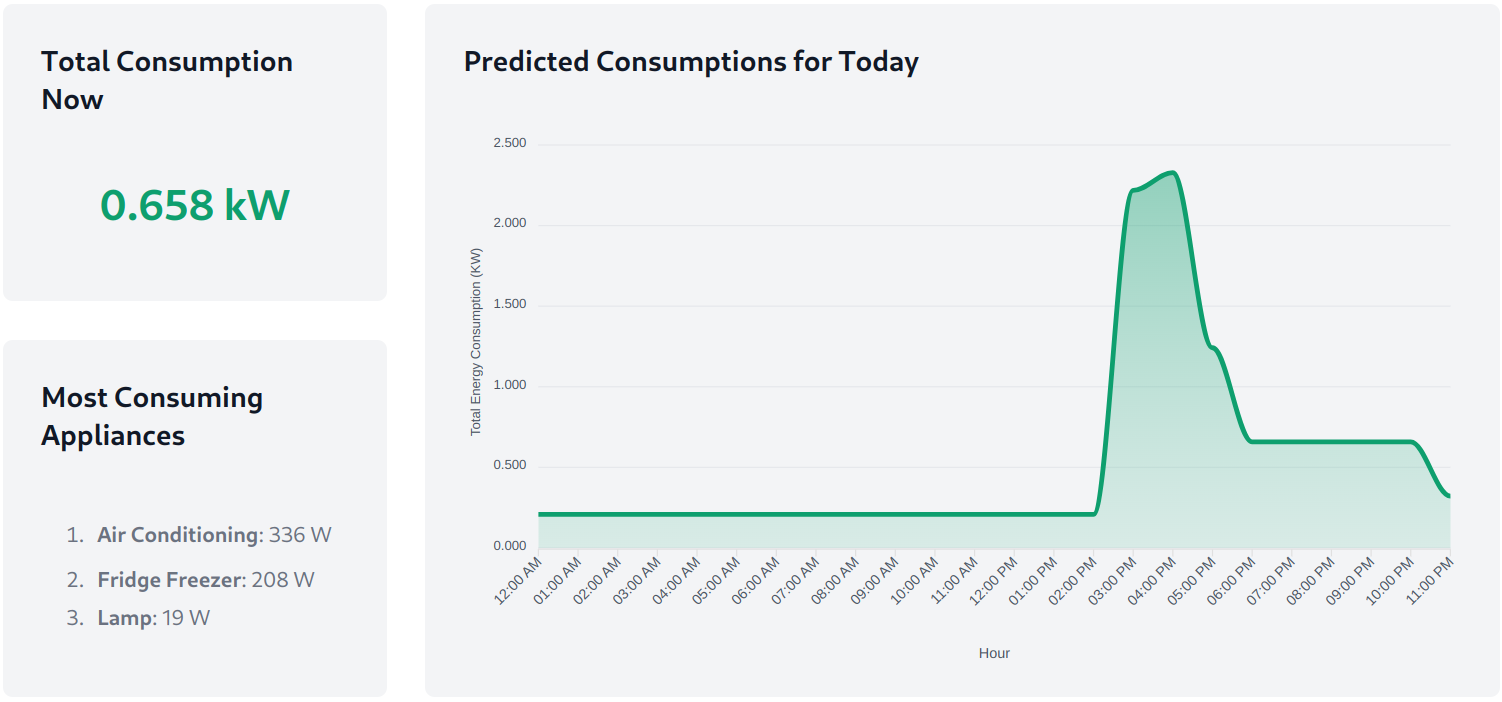
\includegraphics[width=0.9\textwidth]{images/frontend/statistics.png}
    \caption{Statistics section of the frontend application}
    \label{fig:frontend_statistics}
\end{figure}

\subsection{Simulate Section}

The simulate section, depicted in Figure~\ref{fig:frontend_simulate}, allows the user to simulate the effect of adding a new routine to the home, and to detect any potential conflicts with the existing routines. The user can choose from three predefined routines, which illustrate the different outcomes of the simulation process. The routines are presented in a tab interface, which facilitates the comparison and selection of the desired routine. The results of the simulation are shown at the bottom of the section.

\begin{figure}
    \centering
    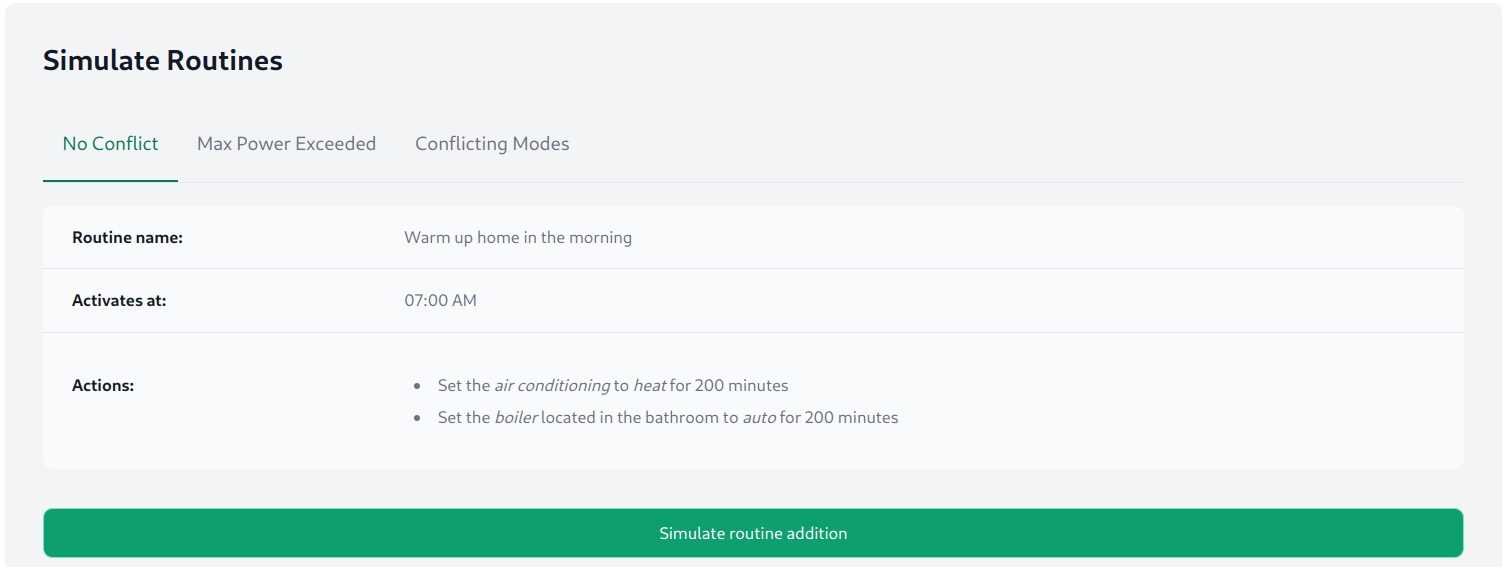
\includegraphics[width=0.9\textwidth]{images/frontend/simulate.png}
    \caption{Simulate section of the frontend application}
    \label{fig:frontend_simulate}
\end{figure}

The "No Conflict" tab, shown in Figure~\ref{fig:frontend_simulate}, displays the details of the "Warm up home in the morning" routine, which activates the air conditioning and the boiler at 7:00 AM. By clicking on the "Simulate routine addition" button, the user can send a \texttt{POST} request to the \texttt{/simulate} endpoint of the \acrshort{api}, and see the result of the simulation in Figure~\ref{fig:frontend_no_conflict_result}. The simulation indicates that the routine is accepted without any conflicts. A graph, which uses the data from the \texttt{/simulate/consumption/total} endpoint of the \acrshort{api}, compares the power consumption with and without the simulated routine. A recommendation to change the start time of the routine to a more optimal one is also provided, along with the projected savings over 30 days.

\begin{figure}
    \centering
    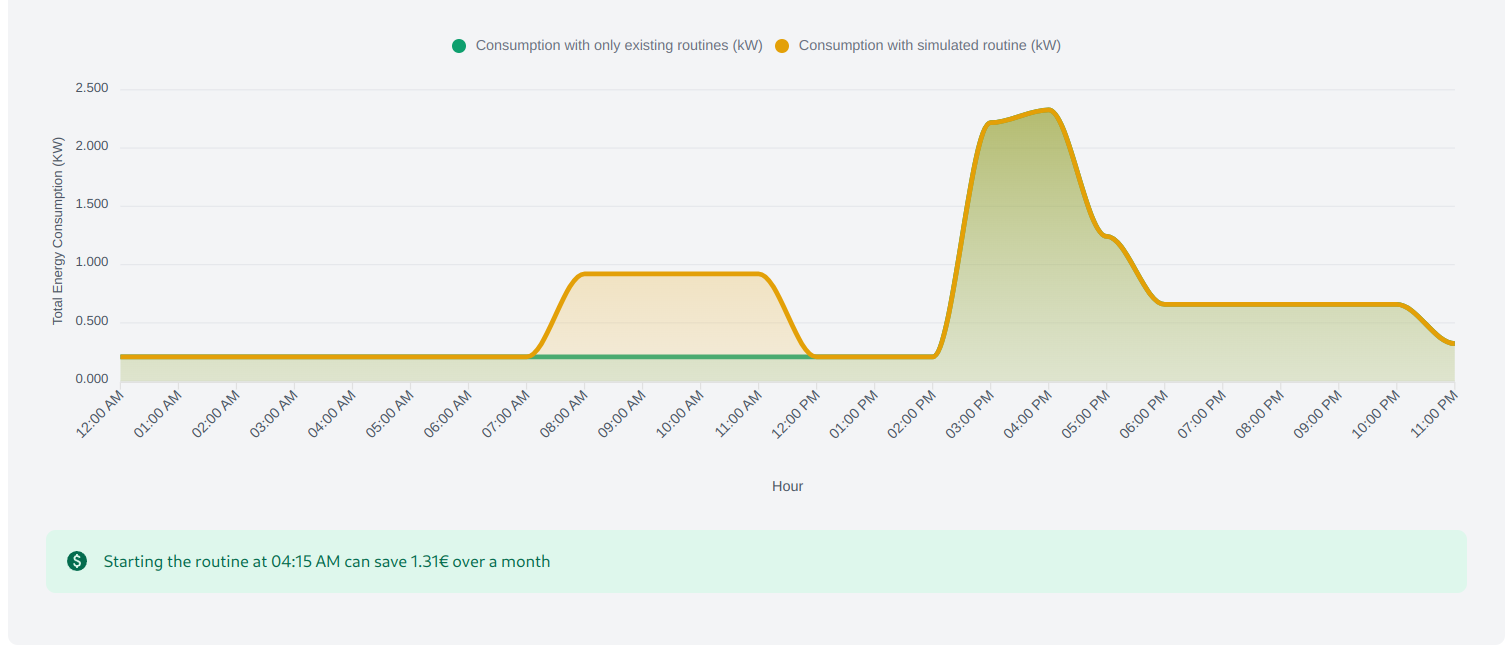
\includegraphics[width=0.9\textwidth]{images/frontend/no_conflict_result.png}
    \caption{Results of simulating the "Warm up home in the morning" routine}
    \label{fig:frontend_no_conflict_result}
\end{figure}

The "Party time" routine, shown in Figure~\ref{fig:frontend_max_power_exceeded}, is designed to test the scenario where the power consumption surpasses the maximum limit of 3kW. It turns on the air conditioning, the dishwasher, the washing machine, and the microwave at 10:00 AM. The simulation results are displayed in Figure~\ref{fig:frontend_max_power_exceeded_result}. The simulation shows an error, due to conflict S2, and suggests disabling either the simulated routine or an existing routine that consumes a lot of power. No recommendation to change the start time of the routine is given, because the routine would always exceed the maximum limit regardless of the time.

\begin{figure}
    \centering
    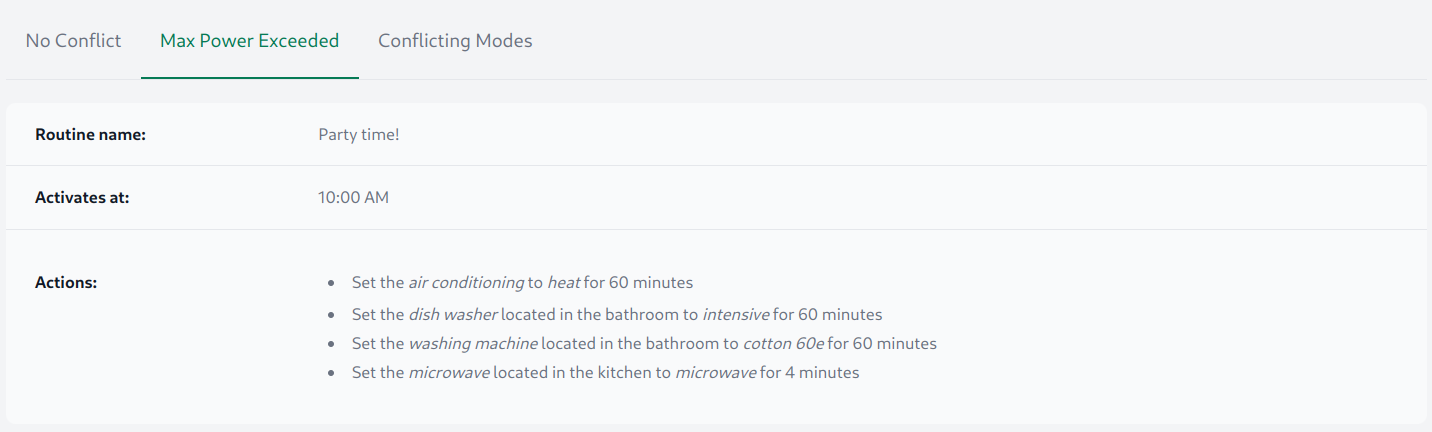
\includegraphics[width=0.9\textwidth]{images/frontend/max_power_exceeded.png}
    \caption{Details of the "Party time" routine, which causes the power consumption to exceed the maximum limit}
    \label{fig:frontend_max_power_exceeded}
\end{figure}

\begin{figure}
    \centering
    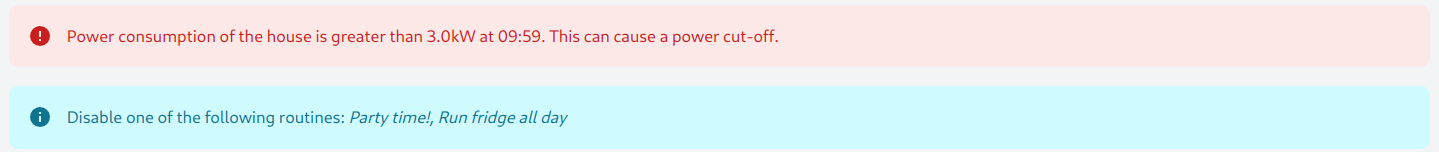
\includegraphics[width=0.9\textwidth]{images/frontend/max_power_exceeded_result.png}
    \caption{Result of simulating the "Party time" routine}
    \label{fig:frontend_max_power_exceeded_result}
\end{figure}

The "Heavy-duty wash" routine, shown in Figure~\ref{fig:frontend_conflicting_modes}, is designed to create a conflict with an existing routine. It sets the washing machine to the \textit{cotton 90} mode at 14:00. However, another routine already sets the washing machine to the \textit{cotton 30} mode at the same time. The simulation results are shown in Figure~\ref{fig:frontend_conflicting_modes_result}. The simulation reports an error, due to conflict S1, and offers two recommendations to disable either of the conflicting routines. A recommendation to change the start time of the routine to a more suitable one is also given, along with the projected savings.

\begin{figure}
    \centering
    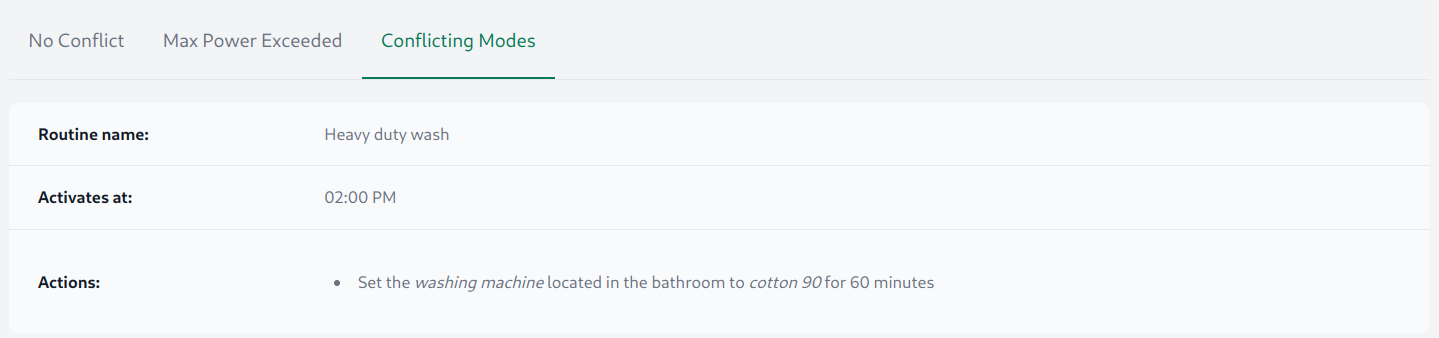
\includegraphics[width=0.9\textwidth]{images/frontend/conflicting_modes.png}
    \caption{Details of the "Heavy duty wash" routine, which causes a conflict with an existing routine}
    \label{fig:frontend_conflicting_modes}
\end{figure}

\begin{figure}
    \centering
    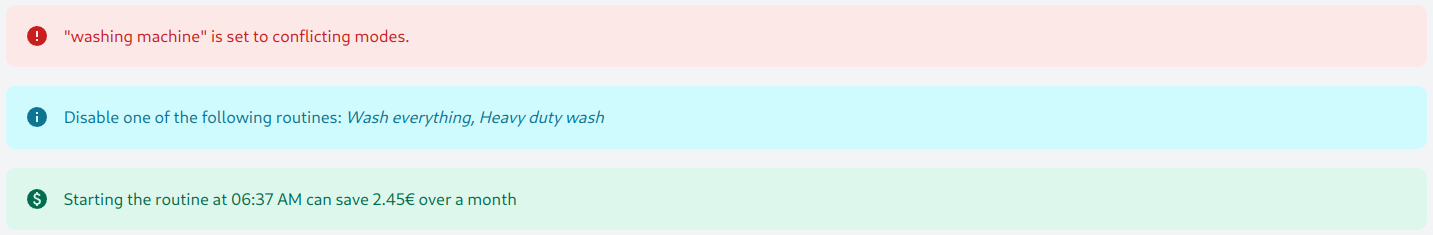
\includegraphics[width=0.9\textwidth]{images/frontend/conflicting_modes_result.png}
    \caption{Result of simulating the "Heavy duty wash" routine}
    \label{fig:frontend_conflicting_modes_result}
\end{figure}

\subsection{Appliances Section}

Figure~\ref{fig:frontend_appliances} shows the appliances section of the frontend application, which displays a table with the device name and type, the manufacturer and model, the location in the home, and the names of the supported operation modes. The table also automatically adds an appropriate icon for each appliance, taken from Material Icons.

\begin{figure}
    \centering
    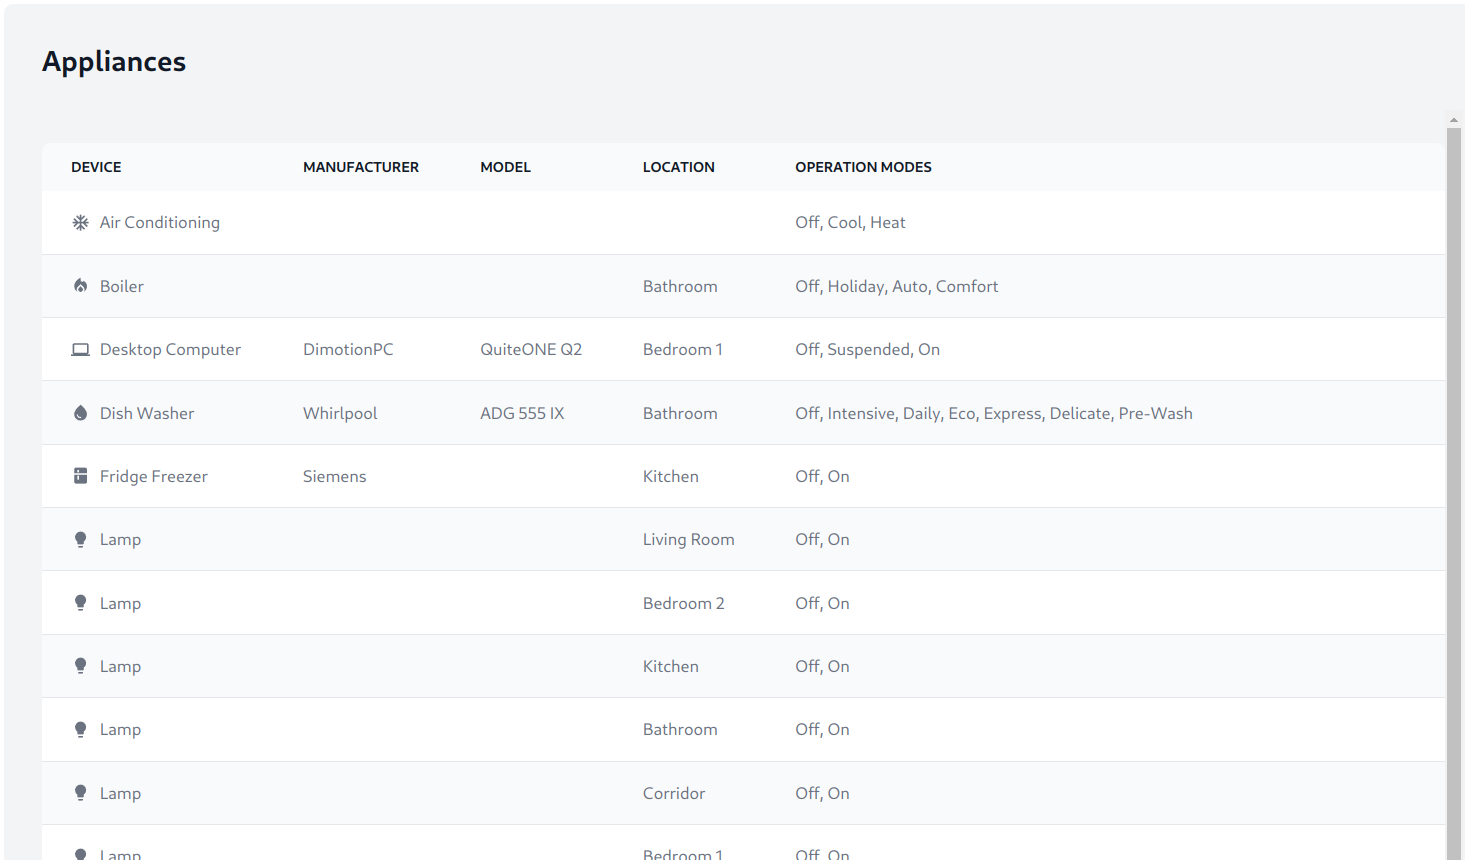
\includegraphics[width=0.9\textwidth]{images/frontend/appliances.png}
    \caption{Simulate Section of the Frontend Application}
    \label{fig:frontend_appliances}
\end{figure}

\subsection{Routines Section}

Figure~\ref{fig:frontend_routines} shows the routines section of the frontend application, which displays a table similar to the one for the appliances. It includes information about the name, time of activation of the routines, whether the routine is enabled or not, and the list of actions of the routines.

\begin{figure}
    \centering
    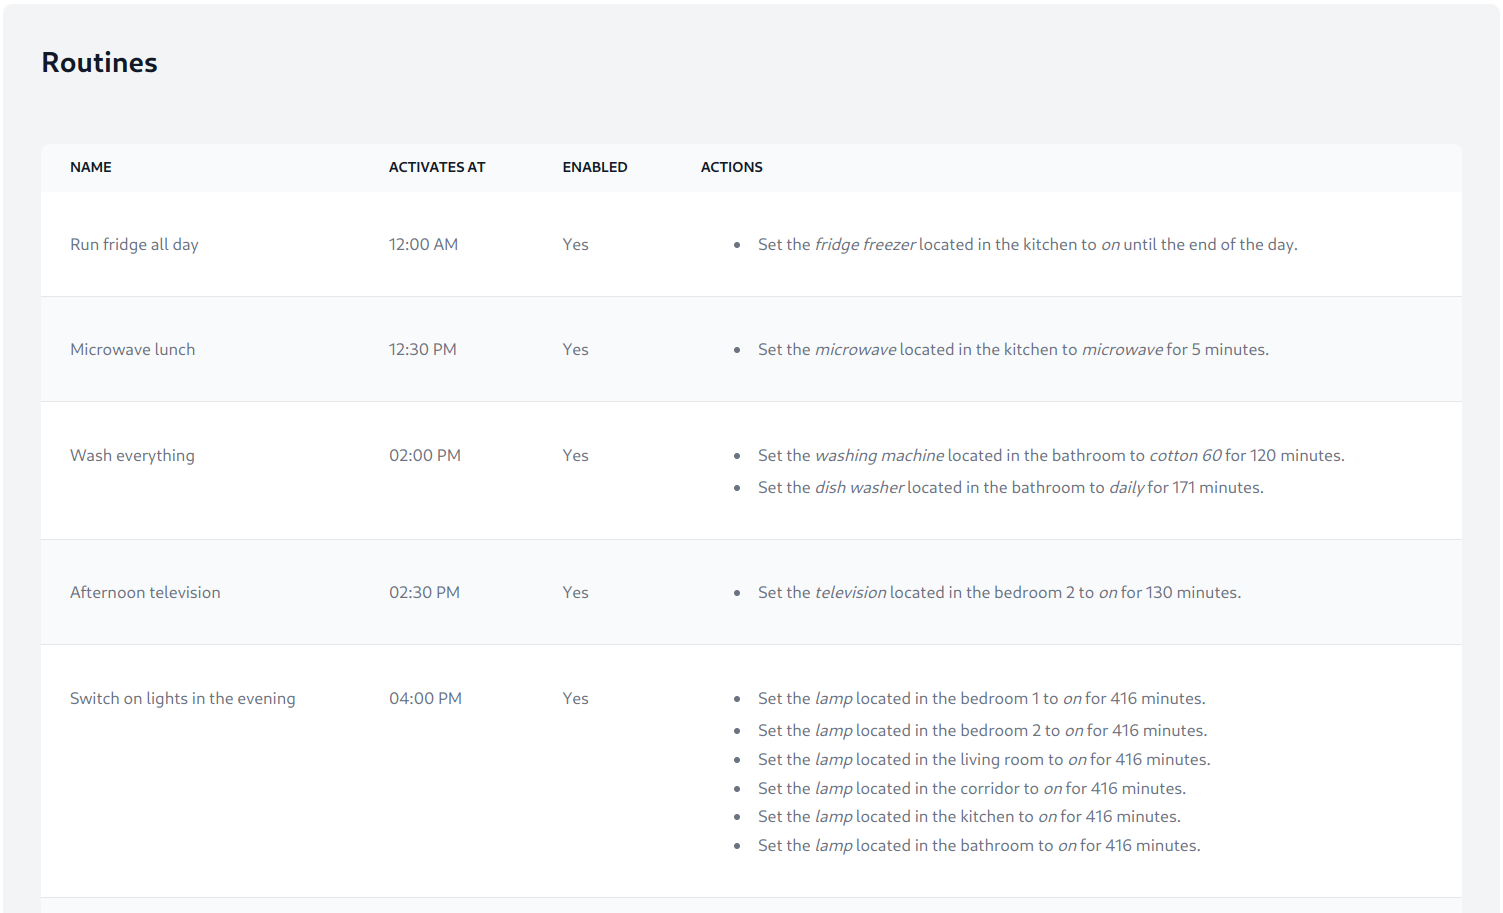
\includegraphics[width=0.9\textwidth]{images/frontend/routines.png}
    \caption{Showcase Frontend Application}
    \label{fig:frontend_routines}
\end{figure}